
In this section we derive our version of the standard quadrotor dynamic model given in \cite{hoffmann2004stanford} and \cite{pounds2002design}. We also derive a model for power consumption based on existing models for general rotorcraft given in \cite{leishman2006principles}.

\begin{figure}[t]
    \label{QuadDiagram}
	\centering
	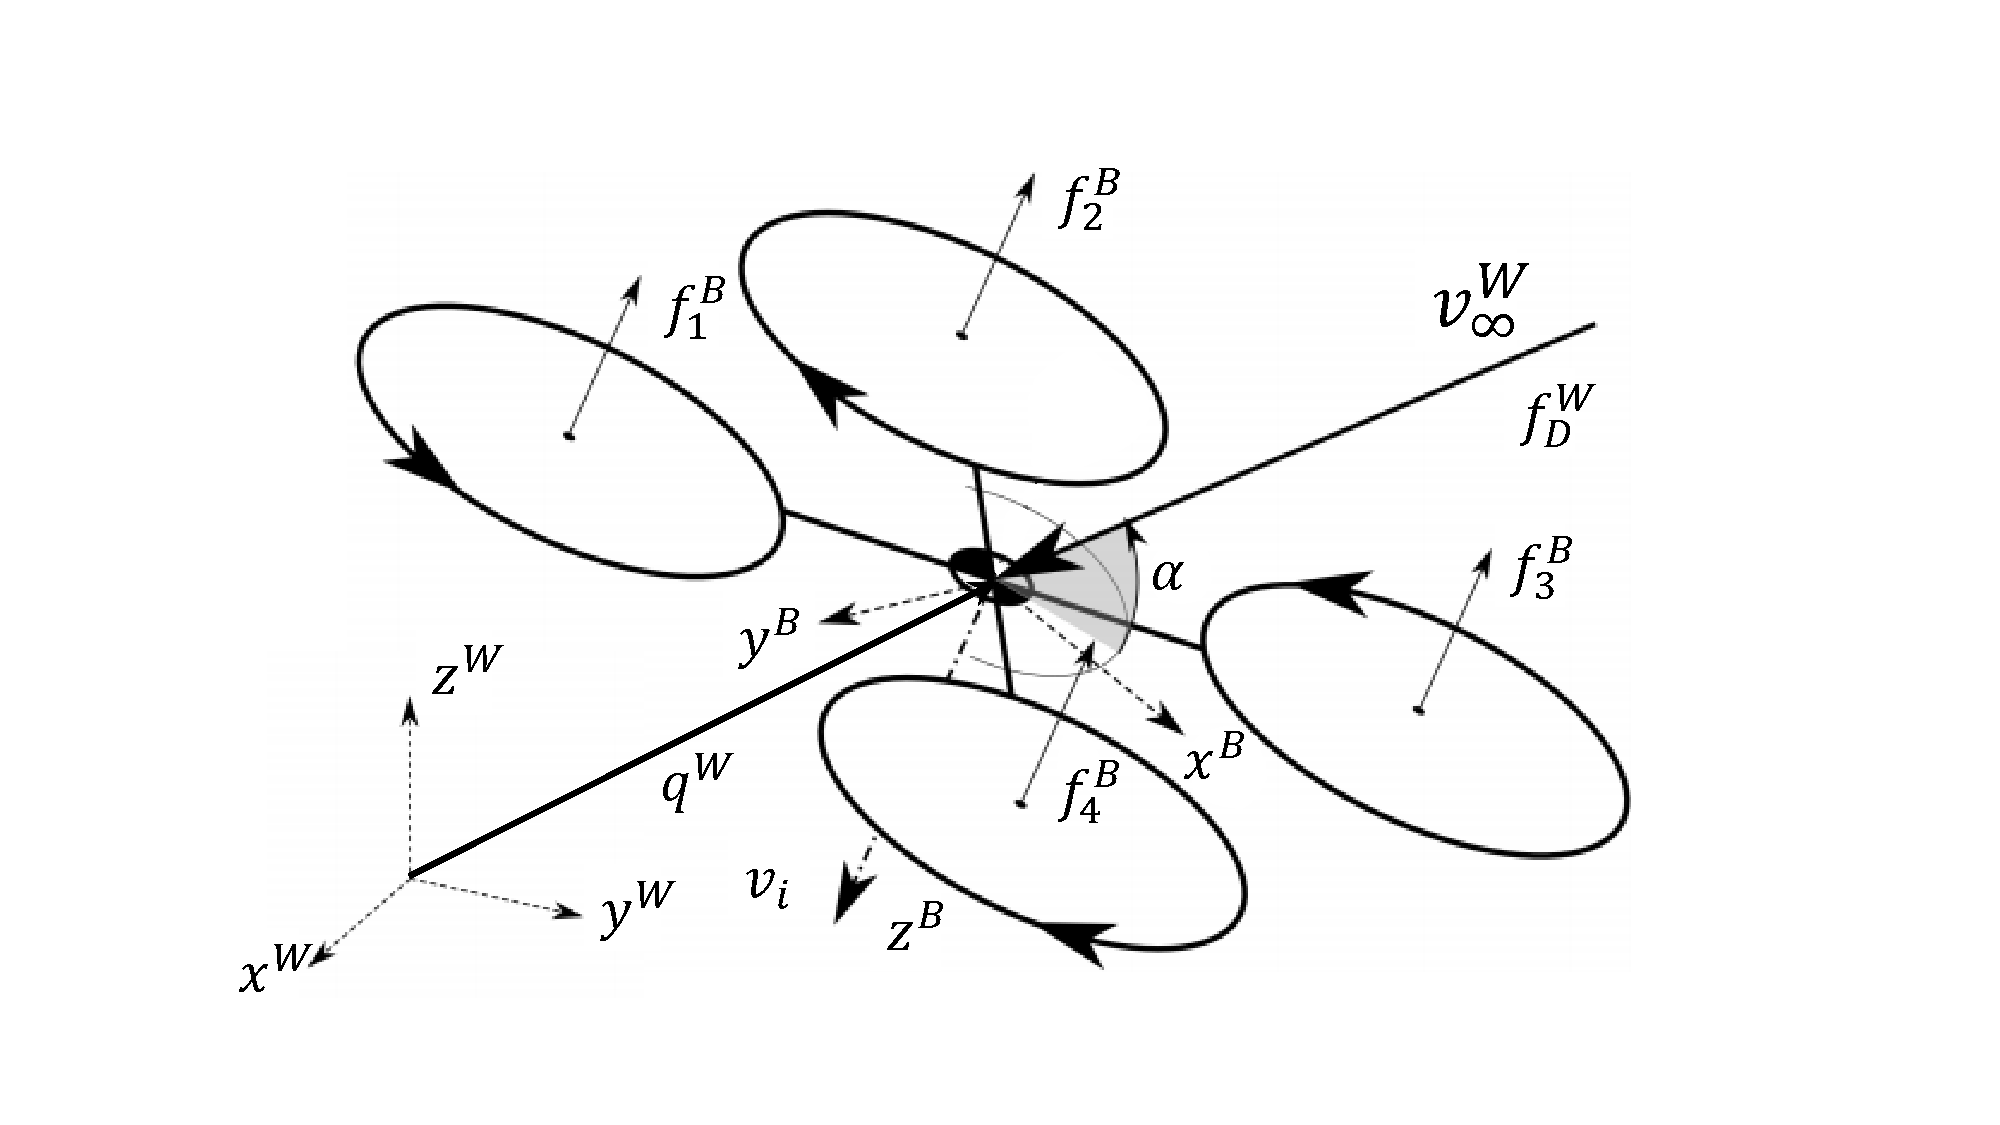
\includegraphics[width=0.5\textwidth, trim={4cm 2cm 5cm 2.5cm},clip]{quad-diagram.pdf}
	\caption{Definition of our coordinate system. Frame $W$ is defined as a NEU inertial frame. Frame $B$ is attached to the quadrotor's center of mass. Keeping with convention, $z^B$ points down so that positive pitch angles, $\theta$, correspond to pitching up. We define $\alpha$ as the angle between $v_\infty^W$ and the plane of the rotors and $v_i$ so that its direction is always equivalent to $z^B$. Diagram adapted from \cite{tagliabue2019model}}
\end{figure}

\subsection{Quadrotor dynamics}
As seen in Fig. 2. we define two frames of reference, $W$ the world or inertial frame and $B$ the body fixed frame attached the quadrotor at its center of mass. We also define $R$, a rotation matrix that describes the orientation of $B$ in $W$; $q^{w}=\left(x^W \text{, } y^W \text{, } z^W\right)$, a vector that gives the Cartesian position of $B$ in $W$; and $\omega_{W,B}^B$, a vector that describes the angular velocity of $B$ with respect to $W$ in the body frame. Since we constrain the quadrotor to always be within $^\pi/_6$ of hover, $R$ can be parameterized by the Euler angles $\Theta^{w}=\left(\phi^W \text{, } \theta^W \text{, } \psi^W\right)$ corresponding to roll, pitch, and yaw respectively.

Assuming all four rotors are identical and neglecting blade flapping then each rotor will produce a thrust $f_j^B \propto \sigma_j$ where $\sigma_j$ is the spin rate of the rotor. Additionally, each rotor will produce a torque, $\tau_j^B$, around each axis of $B$. Torques about $x^B$ and $y^B$ are moments proportional to $\sigma_j$ whereas torques about $z^B$ are pure torques proportional to the difference in spin rate between a rotor and its counter-rotor (i.e. $\sigma_2 - \sigma_4$ and $\sigma_1 - \sigma_3$).

We can then describe the translational and rotational dynamics of the quadrotor as a set of Newton-Euler equations:
\begin{align}
    \label{NewtonEqn}
    m \ddot{q}^W=R\sum{f_j^B}+f_D^W - mg^W
\end{align}

\begin{align}
    \label{EulerEqn}
     I^B\dot{\omega}_{W,B}^B=-\omega_{W,B}^B \times I^B\omega_{W,B}^B+\sum{\tau_j^B}
\end{align}
Where $I^B$ is the rotational inertia matrix, which is diagonal when the quadrotor is axisymmetric, the gravity vector is $g^W=\left(0 \text{, } 0 \text{, } 9.8066\right) \text{ ms}^{-2}$, and $m$ is the mass of the quadrotor in kg.

\subsection{Drag model}
Following \cite{tagliabue2019model} and \cite{schulz2015high} we adopt an isotropic drag model for simplicity.
\begin{align}
    \label{DragEqn}
    f_D^W = \left(\mu_1 v_\infty + \mu_2 v_\infty^2 \right)\frac{v_\infty}{\|v_\infty\|} 
\end{align}
Where $\mu_1$ and $\mu_2$ are experimentally determined drag coefficients selected to make \eqref{DragEqn} approximate a more complex drag model such as the one presented in \cite{huang2009aerodynamics}, \cite{bangura2012nonlinear}, or \cite{leishman2014quadrotors}. As shown in Fig. 2. we assume that $f_D^W$ is always co-linear with $v_\infty$ and acts at the quadrotor's center of mass producing no moments.

\subsection{Power consumption model}
We base our model for power consumption off Leishman's \cite{leishman2006principles} model for aerodynamic power required for level flight and maneuvers. By assuming that the total aerodynamic power required is the sum of the power required to maintain level flight and the power to climb in altitude if needed.
\begin{align}
    \label{PowReqEqn}
    P_{req} = \kappa T \left(v_i + v_\infty^B|_z \right) + \dot{q}^W_z m \|g\|
\end{align}
Where $\kappa$ is an experimentally determined correction factor, $T$ is the sum of all the individual rotor thrusts $f_j$, $v_\infty^B|_z$ is the component of $v_\infty$ orthogonal to the rotor plane, $\dot{q}^W_z$ is the vertical component of the quadrotor's velocity in the world frame, and $v_i$ is the velocity induced by air flowing through the rotors and is defined implicitly by \cite{leishman2006principles} as: 
\begin{align}
    \|v_i\| = \frac{v_h^2}{\sqrt{\left(v_\infty \cos{\alpha} \right)^2 + \left(v_\infty \sin{\alpha} \right)^2}}
\end{align}
where $v_h$ is the induced velocity at hover. This expression for $\|v_i\|$ can be manipulated in to a quartic function and solved numerically \cite{hoffmann2007quadrotor}.

To convert $P_{req}$ to electrical power consumed, $P$, we join \cite{ware2016analysis}, \cite{kreciglowa2017energy}, and \cite{tagliabue2019model} in assuming that all losses due to electrical components can be aggregated in to one efficiency term $\eta$. Thus:
\begin{align}
    P = \frac{1}{\eta} P_{req}
\end{align}
